\documentclass[11pt]{article}
\usepackage[margin=1in]{geometry}
\usepackage{amsmath}
\usepackage{booktabs}
\usepackage{hyperref}
\usepackage{graphicx}
\usepackage{float}
\usepackage{tikz}
\usepackage{longtable}
\usepackage{array}
\usepackage{verbatim}

\title{Inverse Line-Heating Plan Demo: Process, Mathematics, and Results}
\author{}
\date{January 20, 2026}

\begin{document}
\maketitle

\section{Overview}
This document records the inverse planning run for the single-line heating case (plan\_demo), including the mathematical model, the optimization process, a flow chart of the workflow, and the full optimization log. The run targets a midspan deflection profile on a $400\,\mathrm{mm} \times 300\,\mathrm{mm}$ plate of thickness $14\,\mathrm{mm}$.

\section{Mathematical Model}
\subsection{Gaussian Heat Source}
The surface heat flux is modeled as a Gaussian:
\begin{equation}
q(r) = q_0 \exp\left(-\frac{2 r^2}{r_0^2}\right),
\end{equation}
where $r_0$ is the heat source radius. The total power is
\begin{equation}
P = \int_0^{\infty} 2\pi r\, q(r)\, dr = \frac{\pi r_0^2}{2} q_0.
\end{equation}
With line energy input $E_{\mathrm{in}}$ and scan speed $v$, power is $P = E_{\mathrm{in}} v$, giving
\begin{equation}
q_0 = \frac{2 E_{\mathrm{in}} v}{\pi r_0^2}.
\end{equation}

\subsection{Objective}
The planner minimizes a scalar loss between the simulated deflection profile and the target profile. For the single-line case, the target is the midline deflection profile:
\begin{equation}
\{(y_i, w_i)\}_{i=1}^3 = \{(0, 0), (150, 5.8), (300, 0)\}~\mathrm{mm}.
\end{equation}
The reported objective value is the scalar loss returned by the planner for each evaluation.

\section{Process}
\subsection{Inputs}
\begin{itemize}
  \item Plate: $L_x=400\,\mathrm{mm}$, $L_y=300\,\mathrm{mm}$, thickness $14\,\mathrm{mm}$.
  \item Initial line: $y=150\,\mathrm{mm}$, $E=600\,\mathrm{J/mm}$, $v=6\,\mathrm{mm/s}$, 1 pass.
  \item Bounds: $y\in[50,250]$, $E\in[400,1000]$, $v\in[4,20]$, passes $\in[1,3]$.
  \item Solver: Gaussian radius $r_0=7\,\mathrm{mm}$, $\beta=3$, $\Delta t=2\,\mathrm{s}$, extra time $200\,\mathrm{s}$, centerline-fixed boundary condition, inherent strain enabled.
\end{itemize}

\subsection{Workflow (Flow Chart)}
\begin{figure}[H]
\centering
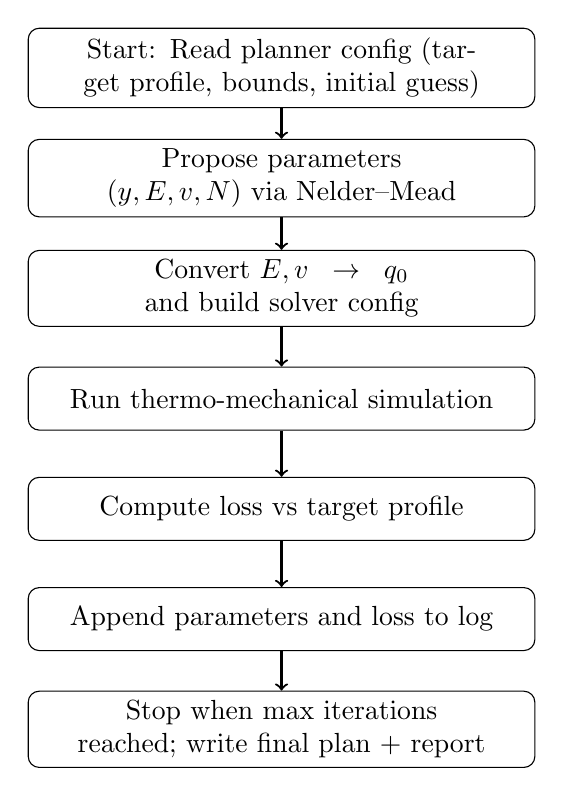
\begin{tikzpicture}[node distance=14mm, align=center]
  \tikzstyle{block} = [rectangle, draw, rounded corners, text width=6.2cm, minimum height=8mm]
  \tikzstyle{arrow} = [->, thick]

  \node[block] (start) {Start: Read planner config (target profile, bounds, initial guess)};
  \node[block, below of=start] (propose) {Propose parameters $(y, E, v, N)$ via Nelder--Mead};
  \node[block, below of=propose] (convert) {Convert $E, v \rightarrow q_0$ and build solver config};
  \node[block, below of=convert] (solve) {Run thermo-mechanical simulation};
  \node[block, below of=solve] (eval) {Compute loss vs target profile};
  \node[block, below of=eval] (log) {Append parameters and loss to log};
  \node[block, below of=log] (stop) {Stop when max iterations reached; write final plan + report};

  \draw[arrow] (start) -- (propose);
  \draw[arrow] (propose) -- (convert);
  \draw[arrow] (convert) -- (solve);
  \draw[arrow] (solve) -- (eval);
  \draw[arrow] (eval) -- (log);
  \draw[arrow] (log) -- (stop);
\end{tikzpicture}
\caption{Inverse planning workflow.}
\end{figure}

\section{Results}
\subsection{Final Plan}
\begin{itemize}
  \item Line position: $y=150.4926\,\mathrm{mm}$
  \item Energy: $E=602.6605\,\mathrm{J/mm}$
  \item Velocity: $v=6.0631\,\mathrm{mm/s}$
  \item Passes: $N=1$
  \item Objective: $3.886\times 10^{-4}$
\end{itemize}

\subsection{Deflection Summary}
\begin{itemize}
  \item $w_{\max}=5.8341\,\mathrm{mm}$
  \item $w_{\min}=-0.5943\,\mathrm{mm}$
  \item Edge-to-edge camber: $0.0847\,\mathrm{mm}$
\end{itemize}

\section{Optimization Log (CSV)}
\footnotesize
\begin{verbatim}
"y_lines,energy,velocity,passes,loss
150.000,600.0,6.0,1,0.2674439275059965
157.500,600.0,6.0,1,279.8982870398637
150.000,630.0,6.0,1,0.2675779865828945
150.000,600.0,6.300000000000001,1,0.2673187025599204
150.000,600.0,6.0,1,0.2674439275059965
142.500,615.0,6.15,1,35.74966759527978
146.250,611.25,6.112500000000001,1,0.565232579905753
153.750,603.75,6.0375,1,0.2602142055874506
157.500,600.0,6.0,1,279.8982870398637
151.875,571.875,6.168749999999999,1,351.8480264009736
150.469,615.46875,6.0421875,1,0.045316937491698524
152.109,609.609375,6.18984375,1,17.636512234386075
150.527,602.40234375,6.0474609375,1,0.0026953082377871667
152.373,610.810546875,6.213574218749999,1,7.608153306374992
150.593,602.70263671875,6.053393554687499,1,0.2988737150738424
150.498,608.935546875,6.04482421875,1,0.039786864196527695
152.139,603.076171875,6.04248046875,1,3.900851874313197
150.264,601.201171875,6.1737304687500005,1,118.89343176598744
150.264,601.201171875,6.02373046875,1,119.39139579188925
151.450,606.6064453125,6.1305175781250005,1,6.931908632698757
152.043,609.30908203125,5.9589111328125,1,9.570380105797188
151.599,607.2821044921875,6.012615966796876,1,18.39362662127945
150.513,605.6689453125,6.046142578125,1,0.06295851505641144
151.333,602.7392578125,6.044970703125,1,0.08792499653271135
150.989,604.50439453125,6.0889892578125,1,1.3690626485726165
150.396,601.8017578125,6.110595703125,1,0.09054067915845421
150.396,601.8017578125,6.035595703125001,1,0.09059788579903823
150.544,602.4774169921875,6.048944091796876,1,0.2530237664975905
150.520,604.03564453125,6.0468017578125,1,0.0035142307379910694
150.930,602.57080078125,6.046215820312501,1,0.39381244057011533
150.461,602.10205078125,6.0790283203125,1,0.002102296060714774
150.758,603.453369140625,6.06822509765625,1,0.015709894874078898
150.203,603.4259033203125,6.074542236328124,1,1.1868372736833357
150.748,602.7845764160156,6.053297424316407,1,0.3787821931853094
150.385,603.2121276855469,6.067460632324218,1,17.371443108645124
150.658,602.8914642333984,6.0568382263183596,1,0.004453024691305696
150.325,602.2623825073242,6.0468395233154295,1,3.680429116977701
150.650,603.1556224822998,6.062878704071045,1,3.3105156928305512
150.494,602.252197265625,6.063244628906251,1,0.027303096598646038
150.491,603.06884765625,6.0629150390625,1,0.0017116578511622259
150.560,602.4967575073242,6.06793327331543,1,98.59386117204912
150.610,602.7777099609375,6.073626708984375,1,0.007864754390014989
150.469,602.603645324707,6.071474075317384,1,0.07302400961717674
150.491,602.5769233703613,6.070588874816895,1,0.0893977186461592
150.476,602.58544921875,6.0709716796875,1,0.03896374943637905
150.550,602.9232788085938,6.068270874023438,1,871.0525289406584
150.493,602.6605224609375,6.063079833984375,1,0.0003886352887343654
150.525,602.7828025817871,6.065424156188965,1,0.003995929848049464
150.442,602.6255321502686,6.062924480438231,1,0.39824362071682273
150.469,602.6999688148499,6.064261078834534,1,0.011412370864593133
150.513,603.0206215381622,6.056868374347686,1,0.01745055293145401
150.504,602.9118284583092,6.060394200682639,1,1.6218173184134512
150.492,602.8646850585938,6.062997436523437,1,0.0022250162233328212
150.509,602.7216625213623,6.06425199508667,1,0.6866915349344552
150.481,602.6802456378937,6.063670456409454,1,0.03278669345189104
150.484,602.6229858398438,6.067025756835937,1,0.27436495096454955
"\end{verbatim}

\section{References to Generated Artifacts}
\begin{itemize}
  \item Plan JSON: \texttt{results/plans/plan\_demo.json}
  \item Simulation summary: \texttt{results/plans/plan\_demo/summary.json}
  \item Report PDF: \texttt{results/plans/plan\_demo/report.pdf}
  \item Optimization log: \texttt{results/plans/plan\_log.csv}
\end{itemize}

\end{document}
